\section{Tracking User Styles across Clear and Dark Web Forums}
\label{chp:stylometry_extensions:followingTrail}
The code to reproduce the following analysis is available on Github at the following URL:\\
 {\url{https://github.com/pranavmaneriker/ccc_darkweb_stylometry}}.

\subsection{Motivation}
\label{chp:stylometry_extensions:followingTrail:motivation}
In~\chapref{chp:sysml}, we described an architecture utilizing text CNNs~\citep{kim2014convolutional} for generating the textual component of representations for authorship attribution on darknet forums.
Recent work on generalizing authorship representations has focused on a variation of the popular sentence transformer architecture~\citep{reimers2019sentencebert}.
Specifically, \citet{riverastao2021learning} compared the transferability of author representation learning models between Amazon reviews, fanfiction short stores, and Reddit comments.
They found that in a zero-shot setting, i.e., without any addition in domain data, the models trained on Reddit data had the highest degree of generalization to new domains.
This work motivates us to explore the generalization capabilities of models trained on clear web data to dark web forums.
We explore two research questions.
First, can we apply author representation models trained on Reddit forum data directly to Darkweb forums?
Second, can we combine data from the dark web and clear web to build better models?

\subsection{Datasets}
\label{chp:stylometry_extensions:followingTrail:datasets}

\begin{figure}
    \centering
    \begin{subfigure}{0.9\linewidth}
       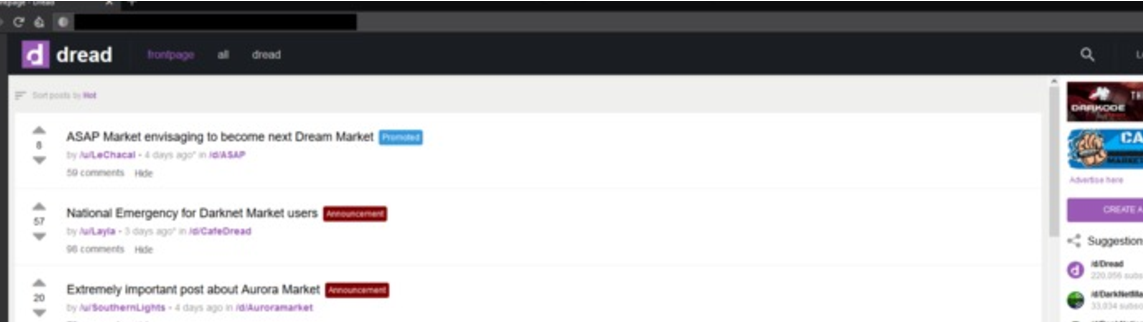
\includegraphics[width=\textwidth]{stylometryExtensions/figures/Dread} 
    \end{subfigure}
    \begin{subfigure}{0.9\linewidth}
       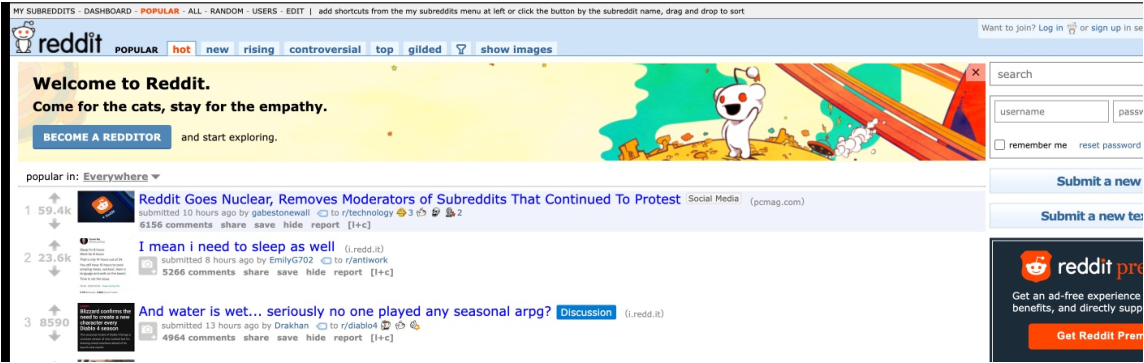
\includegraphics[width=\textwidth]{stylometryExtensions/figures/Reddit} 
    \end{subfigure}
    \caption{Dark web market Dread (top) and clear web market Reddit (bottom). Dread image source:~\citet{wiki:Dread}}
    \label{fig:stylometry_extensions:followingTrail:forums}
\end{figure}

\begin{table}
    \centering
    \begin{tabular}{cccc}
        \toprule
        Dataset &  \# Authors & \# Posts & \# Subforums\\
        \midrule
        Dread & 43,629 & 294,596 & 382 \\
        The Hub & 8,243 & 88,753 & 62 \\
        Reddit-201801 & 4,413,757 & 82,531,775 & 94,945 \\
        Reddit-201912 & 7,439,040 & 126,992,546 & 155,864 \\
        \bottomrule
    \end{tabular}
    \caption{Dataset statistics prior to preprocessing for comparing LUAR on clear and dark web forums.}
    \label{tab:stylometry_extensions:followingTrail:datasets}
\end{table}

To answer the research questions, we collect datasets from both clear and dark web forums.
For the clear web, we sample data from the Pushshift Reddit corpus~\citep{baumgartner2020pushshift}.
The LUAR model is trained on Reddit data sampled from the same corpus, but collected between 2015 and 2019.
To avoid any overlap with the training data, we sample data from 2018 and 2019.
We created two datasets, one for posts sampled from January 2018 and the second for posts sampled from December 2019.
Reddit is an `omni-forum'~\citep{munksgaard2016mixing}, where users can participate in a number of subcommunities (subreddit).
The similarity between Dread and Reddit is illustrated in Figure~\ref{fig:stylometry_extensions:followingTrail:forums}.
Keeping this in mind, we collect `omni-forums' from dark web data.
We collected datasets provided in the CrimeBB collection~\citep{pastrana2018crimebb} and sample data from `Dread' (the dark web version of Reddit) and `TheHub'.
The data from `Dread' is collected between February 2018 and January 2020, and `TheHub' is collected between January 2014 and August 2019.
Summary statistics for the unprocessed datasets are provided in Table~\ref{tab:stylometry_extensions:followingTrail:datasets}. 
As with prior analyses from~\chapref{chp:sysml}, we assume that each username corresponds to a unique author.

\subsubsection{Characterizing Author Behaviors}
\label{chp:stylometry_extensions:followingTrail:datasets:behaviors}

\begin{figure}
    \begin{subfigure}{0.75\linewidth}
        \centering
        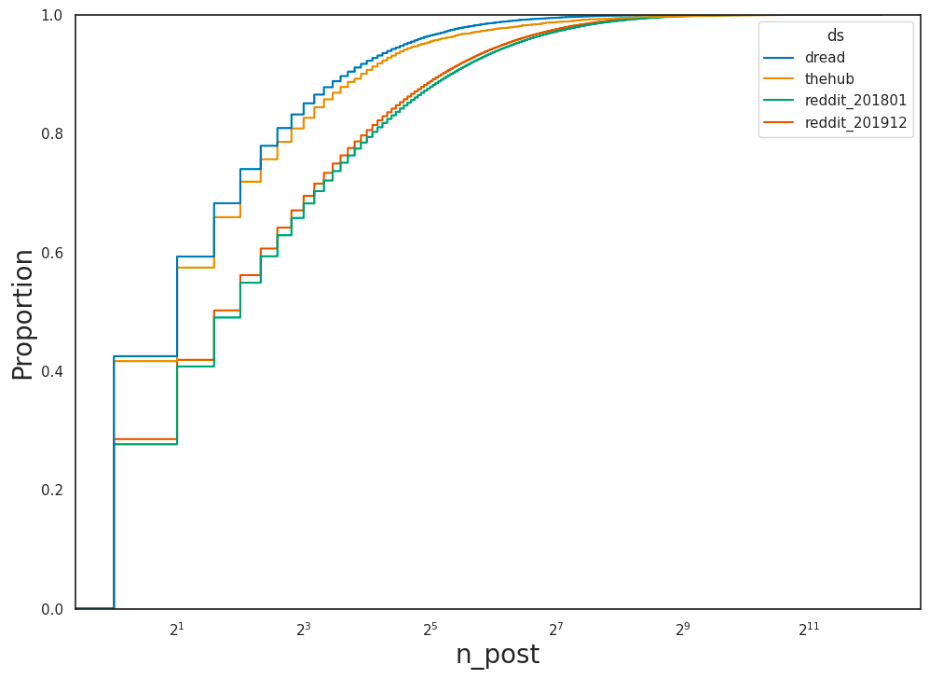
\includegraphics[width=\textwidth]{stylometryExtensions/figures/RedditPostCDF}
        \caption{Empirical Cumulative Distribution Function showing the proportion of authors having n\_post posts. Reddit has a much smaller proportion of authors with only one post.}
        \label{fig:stylometry_extensions:followingTrail:datasets:behaviors:posts}
    \end{subfigure}
    \begin{subfigure}{0.75\linewidth}
        \centering
        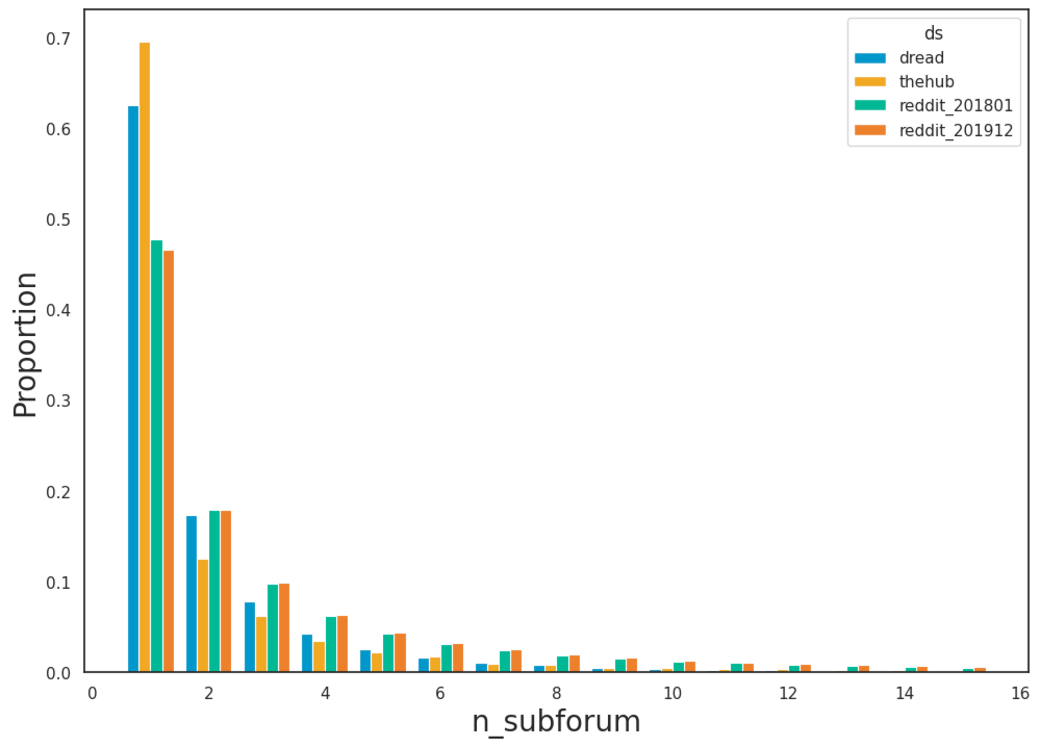
\includegraphics[width=\textwidth]{stylometryExtensions/figures/RedditSubforumCounts}
        \caption{Histogram of the number of subforums an author has posted in. Reddit has fewer authors posting on only one subforum.}
        \label{fig:stylometry_extensions:followingTrail:datasets:behaviors:subforums}
    \end{subfigure}
    \caption{User behaviors on Reddit, Dread, and TheHub.}
    \label{fig:stylometry_extensions:followingTrail:datasets:behaviors}
\end{figure}

As a first step to understanding the differences in the datasets, we aim to characterize the authors.
Figure~\ref{fig:stylometry_extensions:followingTrail:datasets:behaviors} provides two figures that capture distributions that characterize the user behaviors.
Figure~\ref{fig:stylometry_extensions:followingTrail:datasets:behaviors:posts} shows the cumulative distribution function of the number of posts per author.
We observe that Reddit has a much smaller proportion of authors with only one post.
This indicates that there are a larger proportion of authors posting on Darkweb forums with only a single post.
This may indicate that users create \textit{throwaway accounts}~\cite{leavitt2015throwaway} more frequently on the dark web as they desire greater anonymity.
Figure~\ref{fig:stylometry_extensions:followingTrail:datasets:behaviors:subforums} shows the histogram of the number of subforums a user has posted in.
This indicates that authors on Reddit may have interests in diverse topics, or the granularity of subforums is higher on Reddit.
Thus, even from a summary statistics perspective, there are fundamental differences in author behaviors across the clear and dark web forums.
However, it is unclear how these differences at the macro level will affect the generalization capabilities of LUAR.

\subsubsection{Preprocessing and Setup for Author Identification}
\begin{figure}
    \centering
    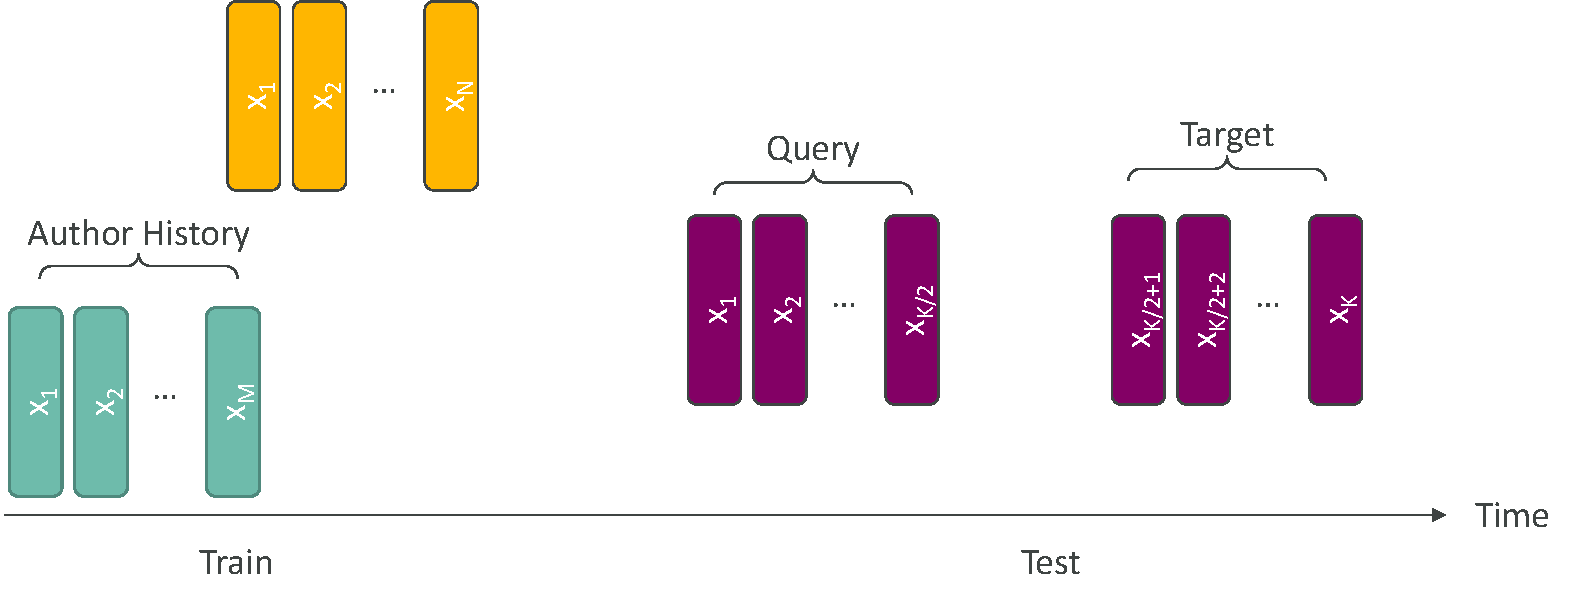
\includegraphics[width=0.9\linewidth]{stylometryExtensions/figures/train_query_target_split}
    \caption{Setup of splits for the Author Identification task. Each color represents a different author.}
    \label{fig:stylometry_extensions:followingTrail:datasets:splits}
\end{figure}
We divide each dataset temporally into a 70-30 split.
That is, the first 70\% of each dataset is used for training models for experiments and the final 30\% is used for evaluation.
The evaluation set is further split into half for constructing a set of query and targets for each author.
Thus, there are three splits for each dataset labeled `train', `test\_query', and `test\_target'.
The models will be evaluated on their ability to match the representation for an author using an episode from the query set against the corresponding one in the target set.
Figure~\ref{fig:stylometry_extensions:followingTrail:datasets:splits} provides a visual representation of the setup for the author identification task. 
We filter the posts to include authors with at least 2 posts and a maximum of 1500 posts.
Further, to control for the significantly higher number of users in the Reddit datasets, we sample authors from Reddit to ensure that there is an equal number of authors in the Dread dataset and each Reddit dataset.
Figure~\ref{fig:stylometry_extensions:followingTrail:datasets:final_splits} shows the number of posts and authors in each dataset and split after preprocessing.


\begin{figure}
    \centering
    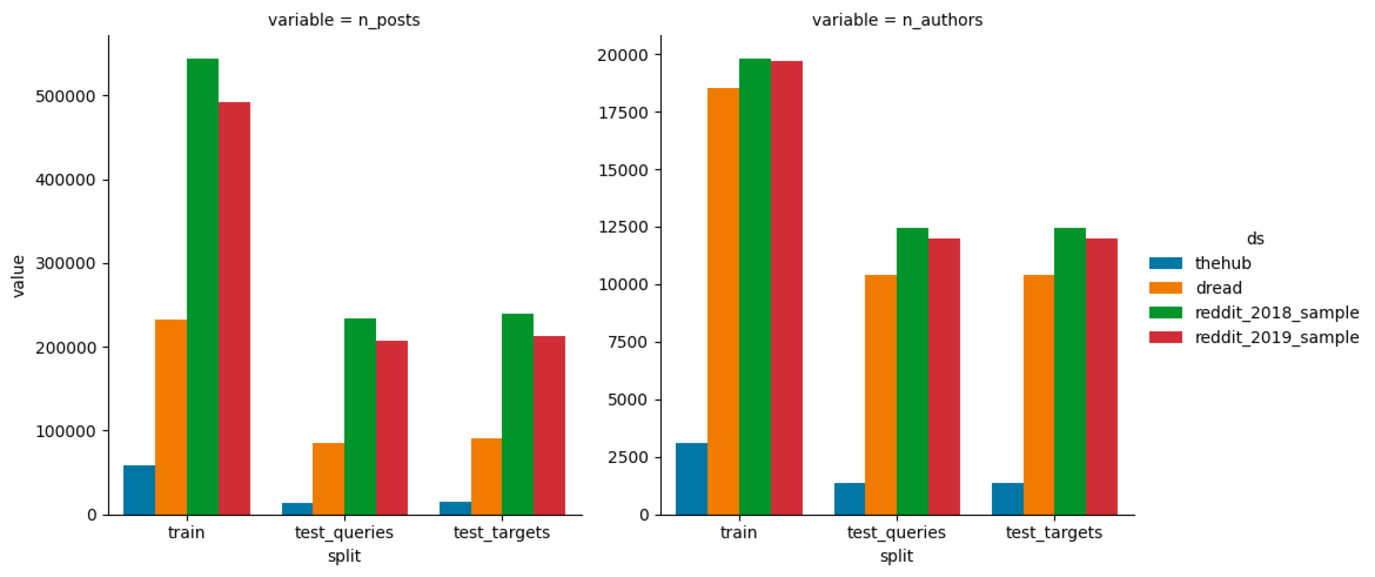
\includegraphics[width=0.9\linewidth]{stylometryExtensions/figures/FinalSplits}
    \caption{Number of authors in each dataset after preprocessing.}
    \label{fig:stylometry_extensions:followingTrail:datasets:final_splits}
\end{figure}

\subsection{Results}

For the following results, we set the episode length to 4. We consider sequence lengths (number of tokens sampled per window) at $32$ and $64$.

\subsubsection{Zero-shot Transfer}
\begin{figure}
    \centering
    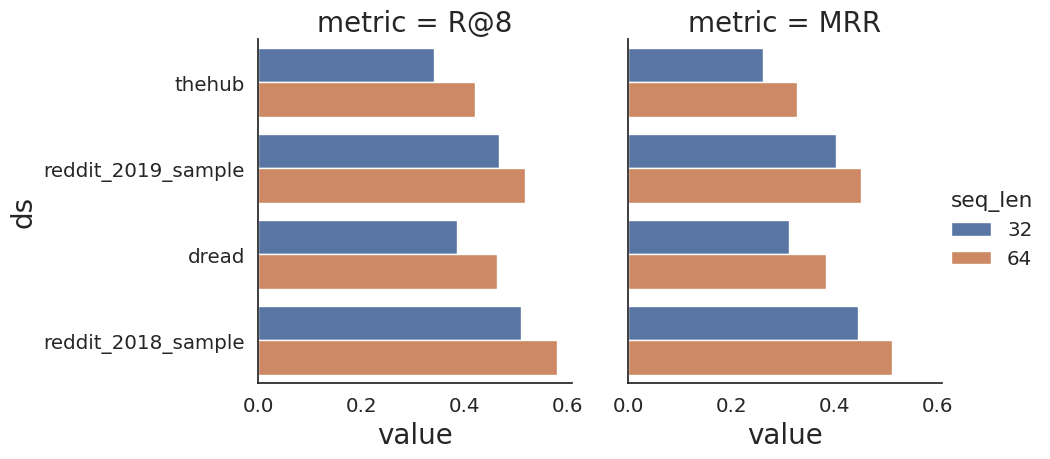
\includegraphics[width=0.9\linewidth]{stylometryExtensions/figures/results/rq1_zeroshot} 
    \caption{Zero-shot performance of LUAR on the test set from Reddit-201801, Reddit-201912, Dread, and TheHub. seq\_len denotes the number of tokens sampled in each window.}
    \label{fig:stylometry_extensions:followingTrail:results:rq1_zeroshot}   
\end{figure}
We first evaluate the original LUAR model \texttt{LUAR-orig} in a zero-shot setting.
That is, we evaluate the model on the test set from the Reddit-201801 and Reddit-201912 datasets, and the Dread and TheHub datasets without any additional tuning.
Figure~\ref{fig:stylometry_extensions:followingTrail:results:rq1_zeroshot} shows the results of this experiment.
We evaluate the Recall@8 and Mean Retrieval Rank (MRR) for the LUAR model (see Section~\ref{sec:sysml:eval} for definitions of these metrics).
The results show that the LUAR model performs well on the Reddit datasets (R@8 $>0.5$ for a sequence length of $64$), but has a significant drop in performance on the Dread and TheHub datasets.
This indicates that a zero-shot transfer of the LUAR model from Reddit to Dread and TheHub is not sufficiently effective.
For the remainder of the experiments, we use the sequence length of $64$ as it provides the best performance on the Reddit datasets.

\subsubsection{Darkweb vs Clearweb Models}
\begin{figure}
    \centering
    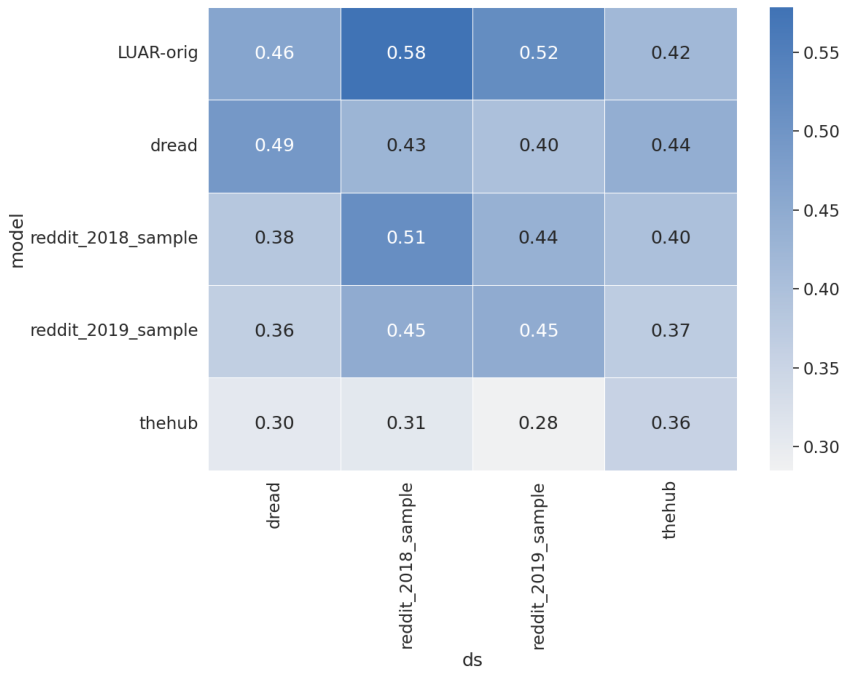
\includegraphics[width=0.8\linewidth]{stylometryExtensions/figures/results/rq2_trainedmodels} 
    \caption{Heatmap comparing Recall@8 across models. Each row represents the training dataset used for training the LUAR model, while each column represents the test dataset.}
    \label{fig:stylometry_extensions:followingTrail:results:rq2_trainedmodels}
\end{figure}
To better understand the impact of different datasets, we train a separate LUAR model on the training split of each of the datasets.
The heatmap in figure~\ref{fig:stylometry_extensions:followingTrail:results:rq2_trainedmodels} shows the results of this experiment.
Each row corresponds to the dataset used to train the LUAR model, and each column corresponds to the test dataset.
The first row corresponds to the results from the original LUAR model trained on one year of Reddit data.
We find that the Dread-based training dataset is significantly better than the Reddit-based training datasets for generalizing to stylometry on Darkweb data.
In fact, the performance of the model trained on Dread generalizes better to TheHub than the model trained on one full year of Reddit data.
At the same time, we note that the Dread-based model falls short of the Reddit-based models on the Reddit datasets.
This motivates us to try a hybrid approach, where we train the LUAR model on a combination of Reddit and Dread data.

\subsubsection{Hybrid Dataset: Combining Clear and Dark Web Data}
\begin{figure}
    \centering
    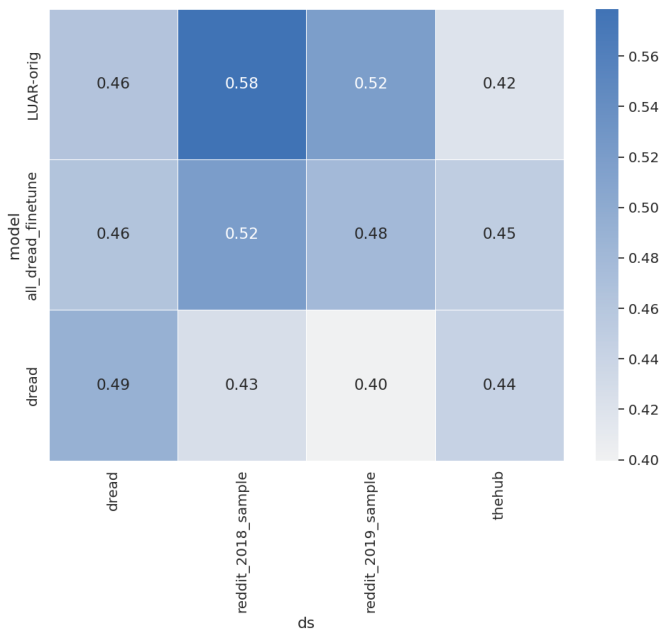
\includegraphics[width=0.8\linewidth]{stylometryExtensions/figures/results/rq3_combine} 
    \caption{Heatmap comparing Recall@8 across models with a combined dataset and individual datasets.}
    \label{fig:stylometry_extensions:followingTrail:results:rq3_combine}
\end{figure}

Finally, in Figure~\ref{fig:stylometry_extensions:followingTrail:results:rq3_combine}, we evaluate the performance of the LUAR model trained on a combination of Reddit and Dread data.
The R@8 for this model improves upon the R@8 of the models trained on Reddit or Dread alone in its ability to generalize to TheHub.
This supports our hypothesis that combining data from the clear and dark web can lead to better generalization capabilities for author identification models.

\subsection{Discussion}
The results of the experiments show that the LUAR model trained on Reddit data alone does not generalize well to darkweb datasets (Dread and TheHub).
However, creating a hybrid dataset by combining data from Reddit and Dread leads to better generalization capabilities.
This supports our thesis that combining data from the clear and dark web can lead to better generalization capabilities for author identification models.
Further work in this direction could explore the impact of different proportions of clear and dark web data on the generalization capabilities of author identification models.


\endinput